\documentclass[a4paper, 11pt]{article}
\usepackage{graphicx}
\usepackage{tabularx}
\begin{document}
We used the \textsc{Stride} threat model to analyze how a package manager of a particular distribution interacts with the main or an official mirror repository. See figure \ref{fig:model}.\\
For most open source distributions of \textsc{Linux}, it is possible for a third party user to set up a mirror server and request to be added to the official list of official servers. After the submission of the request, an administrator of the \textsc{Linux} distribution will verify that the mirror server respects the guidelines of the distribution and eventually accept or dismiss the request.\\
If the request to be added to the official list of mirrors is granted, clients can access this server to install packages.
From our threat model analysis we summarized the existence of 5 types of attacks that can be conducted by a malicious mirror. The following tables summarizes these attacks and the type of threats they cause.
\linebreak
\begin{center}
\begin{tabularx}{\textwidth}{|X|X|X|}
\hline
Type & Description & Threats \\
\hline
Arbitrary Package & In this case the mirror will provide the a package that is the different from the the package the client wants.
& Tampering\\
\hline
Replay Attack & The mirror provides an older version of packages. This might harm the clients as they will be installing versions which might not contain the latest security patches. & Tampering and threats contained in the previous release of the package\\
\hline
Freeze attack & This type of attack is similar to the previous attack. But in this case the attacker modifies the metadata by providing one that is not correct. & Tampering and threats contained in the previous release of the package \\
\hline
Extraneous Dependencies & Attack modifies metadata to add other dependencies. & Tampering \\
\hline
Endless Data & The mirror server returns infinite stream of data to the client package manager. & Denial of service \\
\hline
\end{tabularx}
\end{center}

\begin{figure}
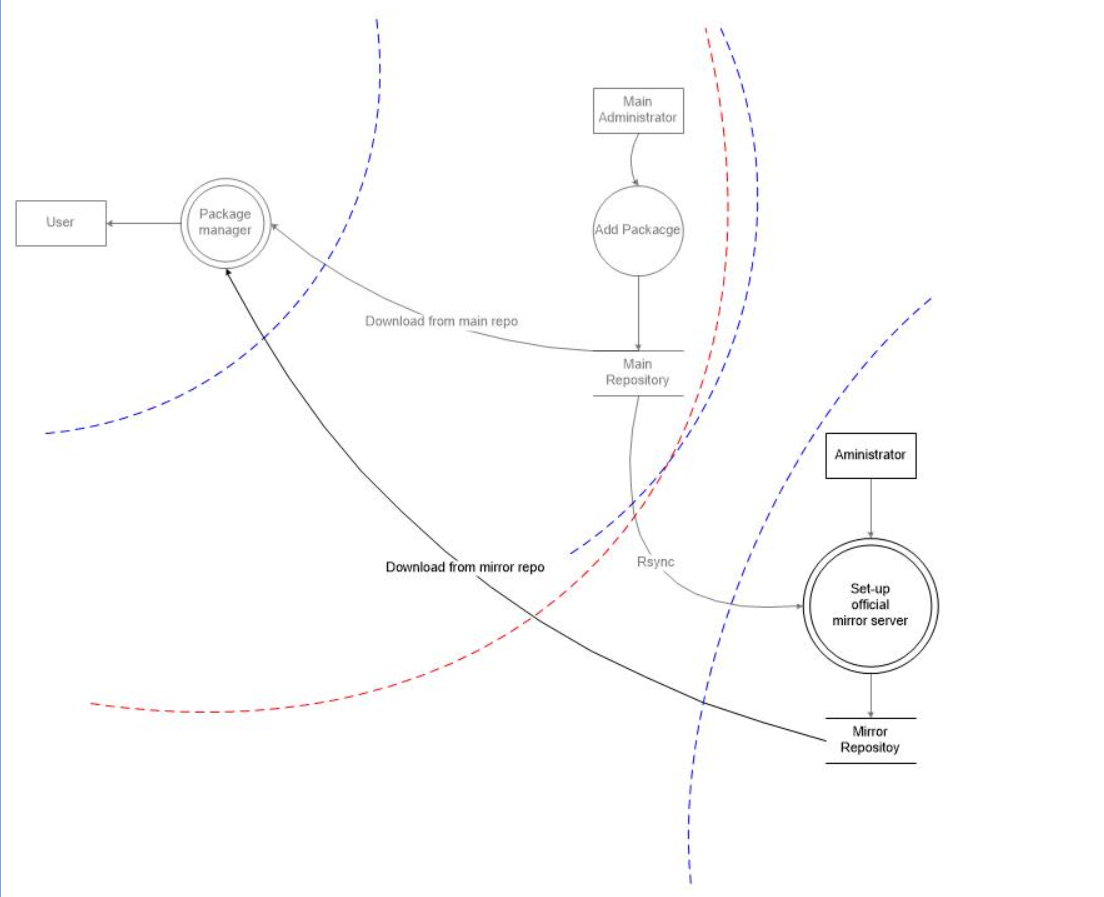
\includegraphics[scale=0.5]{model.png}
\label{fig:model}
\end{figure}
\end{document}\begin{tabular}{|r|r|}
 